\documentclass{emulateapj}
\bibliographystyle{apj}

%define general packages
\usepackage{epsfig}
\usepackage{rotating}
\usepackage{amsmath}
\usepackage{natbib}
\usepackage{footnote}
\usepackage{courier}

%internal short cuts
\def \HgA {H$\gamma_A$}
\def \gon {Gonz\'{a}lez}
\def \Hbp {H$\beta ^\prime$}

\begin{document}

\title{PRIMUS: Quiescent Fraction as a Function of Environment and Redshift}
\author{ChangHoon Hahn, Michael Blanton, Alison Coil, Richard Cool, Daniel Eisenstein, John Moustakas, Ken Wong, Guangtun Zhu}

\begin{abstract}
We examine the evolution of the quiescent fraction ($f_{\rm{Q}}$) for galaxies in 
different density environments from $z=0.0-0.8$ using spectroscopic 
redshift and multi-wavelength imaging data from PRism MUlti-object 
Survey (PRIMUS) and the Sloan Digitial Sky Survey (SDSS). We construct 
a stellar mass limited target galaxy population of 
$40430$ galaxies from PRIMUS within the redshift range $0.2-0.8$ and $106732$
galaxies from SDSS within redshift range $0.0375-0.145$. We classify  
these target galaxies as quiescent or star-forming using an evolving cut 
based on specific star formation rate (SSFR). For each of these galaxies 
we also measure its environment using a fixed cylindrical aperture method 
on a volume-limited {\em Environment Defining Population} constructed
from PRIMUS and SDSS. Based on its environment measurements we classify our target
population into high or low density environments.   

With the target galaxy population divided into quiescent and star-forming galaxies 
in high and low density environments, we calculate the stellar mass functions 
(SMFs) for each of these subsamples. Over the redshift range $z=0.8$ to $0.0$, 
in high density environments we find that the SMFs of the quiescent galaxies 
increase by a factor of $over9000$ for $\mathcal{M}_{*} < 11.0$ while the SMF 
of the star-forming galaxies evolves little for all masses. Meanwhile in low 
density environments from $z=0.8$ to $0.0$, we find that the SMF of quiescent 
galaxies evolves little for all stellar masses and the SMF of star-forming 
galaxies decreases by a factor of $over9000$ for $\mathcal{M}_{*} > 10.5$.  
Furthermore, we compute the $f_{\rm{Q}}$s using the SMFs in the subsamples to 
examine the evolution of the $f_{\rm{Q}}$ in high and low density environments
over the redshift range. We find that at $\mathcal{M}_{*} \sim 10.5$, $f_{\rm{Q}}$ 
increases by $\sim 0.15$ from $z=0.8$ to $0.0$ for both high and low environments. 
In addition, throughout the entire redshift range the difference between the
$f_{\rm{Q}}$ at high and low environment remains constant at $\sim 0.1$. 
These results suggest that the evolution of $f_{\rm{Q}}$ is independent of environment. 
\end{abstract}

%Section heading
\section{Introduction}
\begin{table*} %Subject to significant change based on the classification of environment
  \caption{Summary of Galaxy Subsample}
  \label{tab:subsample}
  \begin{center}
    \leavevmode
    \begin{tabular}{lllll} \hline \hline              
  Survey    &Redshift ($z$) &Density        &Quiescent $N_{\rm{g}}$ &Star-forming $N_{\rm{g}}$  \\ \hline 
  SDSS      &$0.0375-0.145$ &High           &5470                       &4501                           \\
            &               &Mid            &3614                       &4438                           \\
            &               &Low            &5419                       &8927                           \\
            &               &               &                       &                           \\ \hline
  PRIMUS    &$0.2-0.4$      &High           &322                    &583                           \\
            &               &Mid            &177                    &403                          \\
            &               &Low            &768                    &2516                           \\
            &               &               &                       &                           \\ \hline
  PRIMUS    &$0.4-0.6$      &High           &350                       &675                           \\
            &               &Mid            &195                       &405                           \\
            &               &Low            &871                       &2385                           \\
            &               &               &                       &                           \\ \hline
  PRIMUS    &$0.6-0.8$      &High           &347                       &430                           \\
            &               &Mid            &186                       &327                           \\
            &               &Low            &833                       &1847                           \\
            &               &               &                       &                           \\ \hline
  PRIMUS    &$0.8-1.0$      &High           &136                       &232                           \\
            &               &Mid            &94                       &163                           \\
            &               &Low            &373                       &810                           \\
            &               &               &                       &                           \\ \hline
  \multicolumn{5}{l}{}                                             \\       
    \end{tabular} 
  \end{center}
\end{table*}
Galaxies, in their detailed properties, carry the imprints of their
surroundings, with a strong dependence of the quiescent fraction of
galaxies on their local environment (e.g. \citealt{hubble36a,
oemler74a, dressler80a, hermit96a, guzzo97a}; for a recent review see
\citealt{blanton09a}).  The strength of this dependence is itself a
strongly decreasing function of galaxy stellar mass; at the extreme,
the lowest masses ($<10^{9}$ $M_\odot$) galaxies are quenched only in
dense regions, and never in isolation (\citealt{geha12a}).  These
effects vary with redshift at least in the densest clusters, as
observed in the changing fraction of late-type spirals relative to the
field found in studies of the morphology-density relation
(\citealt{dressler84a, desai07a}).  Clearly understanding the
properties of galaxies in the present-day universe requires a careful
investigation of the role of environment, and how that role changes
over time.

Nevertheless, the evolution of the role of environment is a relatively
subtle effect and difficult to study.  Although history of galaxies
prior to $z\sim 1$ appears to have been one of rapid assembly, since
that time the galaxy population has continued to evolve, but less
dramatically. Although there are detectable changes in the population,
the major classes of galaxies existed at $z\sim 1$, in roughly the
same relative numbers as today (\citealt{bundy06a, borch06a,
taylor09a, moustakas13a}. Furthermore, at those redshifts we can also
detect the dependence of galaxy properties on environment, with lower
star-formation rate early-type galaxies populating the denser regions
(\citealt{cooper08a, patel09a, kovac10a}).

The most dramatic change in galaxy properties during the past eight
billion years has been a remarkable decline in the star-formation rate
of galaxies in the Universe (\citealt{hopkins06a}).  This decline
appears dominated by decreases in the rates of star-formation of
individual galaxies (\cite{Noeske:2007aa}). There is evidence that a
large fraction of the decline associated with strongly
infrared-emitting starbursts (\citealt{bell05a, magnelli09a}).  The
decline does not appear to be due to the quenching of a large
fractions of the star-forming population, as reflected in observations
of the stellar mass function of quiescent and star-forming galaxies
(\cite{Blanton:2006aa},\citealt{bundy06a, borch06a, moustakas13a}).  These
findings leave little room for the participation of
environmentally-driven quenching in the global census of
star-formation.  As \citet{cooper08a} and others have pointed out,
because the environmental dependence of total star-formation rates at
fixed redshift is relatively small, environmentally effects are
unlikely to cause the overall star-formation rate decline.

Thus, the impact of environment on galaxy formation has to be
interpreted on top of the background of this overall decline affecting
galaxies in all environments.  The most straightforward investigation
of would directly determine the star-forming properties of galaxies as
a function of environment, stellar mass and redshift in a single,
consistently analyzed data set. This analysis can reveal how galaxies
are quenched in the universe over time, quantitatively establish the
contribution of environmental effects to the overall trends, and
reveal whether those trends happen equally in all environments.
However, such an analysis has not been done previously due to the lack
of sufficiently large samples. In this paper, we apply this approach
using the Prism Multi-object Survey (PRIMUS; \cite{Coil:2011aa}, 
\cite{Cool:2013aa}), the largest available redshift survey covering the epochs
between $0<z<1$.

\section{Sample Selection}
In this paper we are interested in measuring the evolution of the quiescent 
fraction over a wide range of redshifts and in different galaxy density environments. 
In order construct a sample with redshift depth and robust enough redshift values 
to measure galaxy environment, we use galaxies at intermediate redshifts from PRIMUS. 
Additionally we supplement our sample with galaxies at low redshift ($z \sim 0.1$) from SDSS.

We begin with a brief summary of the PRIMUS data in Section \ref{sec:primus} followed by a summary of the SDSS data in Section \ref{sec:sdss}.
Then in Section \ref{sec:target} we use this data to define the stellar mass complete target galaxy population.
Afterwards, in Section~\ref{sec:sfq}, we classify these target galaxies as quiescent or active star-forming galaxies. 
We then obtain the environment for the target galaxy population using a volume-limited {\em Environment Defining Population} in Section \ref{sec:environment}. 
Finally in Section \ref{sec:edgeeffect}, we impose cuts on the target galaxy environment based on the edges of the survey. 

\subsection{PRIMUS} \label{sec:primus}
For galaxies at intermediate redshifts we use multiwavelength imaging and spectroscopic redshifts data of PRIMUS, which is a faint galaxy survey with precise spectroscopic redshifts ($\sigma_z/(1+z) \approx 0.5 \%$) for $\sim 120,000$ galaxies within redshifts $z \approx 0-1.2$.
The survey was conducted using a IMACS spectrograph on a Magellan I Baade $6.5$ m telescope with a slitmask and low dispersion prism.
For further details on the PRIMUS observation methods, including survey design, targeting, and data summary, we refer readers to the survey papers: \cite{Coil:2011aa} and \cite{Cool:2013aa}.

As done in \cite{Moustakas:2013aa}, we only use fields targeted by PRIMUS with $GALEX$ and {\em Spitzer}/IRAC imaging.
This restricts us to five fields.
Four of these fields are a part of the {\em Spitzer} Wide-area Infrared Extragalactic Survey (SWIRE\footnote{http://swire.ipac.caltech.edu/swire/swire.html} ): 
the European Large Area ISO Survey - South $1$ field (ELAIS-S1\footnote{http://dipastro.pd.astro.it/esis}), the Chanddra Deep Field South SWIRE field (CDFS), 
and the XMM Large Scale Structure Survey field (XMM-LSS).
The XMM-LSS consists of two separate but spatially adjacent fields: the Subaru/XMM-Newton DEEP Survey fied (XMM-SXDSS\footnote{http://www.naoj.org/cience/SubaruProject/SDS})
and the Canadian-France-Hawaii Telescope Legacy Survey field (XMM-CFHTLS\footnote{http://www.cfht.hawaii.edu/Science/CFHLS}).
In addition to the SWIRE fields we also include the COSMOS\footnote{http://cosmos.astro.caltech.edu} field for a total of five fields. 

In all of the PRIMUS target fields we have near-UV (NUV) and far-UV (FUV) measurements from the {\em GALEX} Deep Imaging Survey (DIS; \cite{Martin:2005aa}; \cite{Morrissey:2005aa}). 
To minimize contamination from neighboring sources, we use a Bayesian photometric code EM$_{\rm{PHOT}}$ (based on expectation maximization algorithm of \cite{Guillaume:2006aa}). 
Furthermore, we use ground-based optical and {\em Spitzer}/IRAC mid-infrared photometric catalogs in each of the fields to obtain integrated fluxes in all 
photometric bands.
To summarize, the general strategy employed is to use a circular aperture photometry to constrain the shape of the SED and then fixing the overall normalization to 
a estimate of the total magnitude in the detection band. 
\cite{Moustakas:2013aa} provides a detailed description of the calculation for each of our target fields.  

From the spectroscopic redshift and photometry described above, we use \texttt{iSEDfit} to determine stellar masses, star formation rates (SFRs) and other physical properties
in a simplified Bayesian framework.
\texttt{iSEDfit}, which we will only briefly mention in this paper is discussed in detail in Appendix A. of \cite{Moustakas:2013aa}.
The code uses the redshift and the observed photometry of the galaxies to determine the statistical likelihood of a large ensemble of generated model SEDs. 
These generated model SEDs depend on population synthesis models and prior parameters.
In order to derive our fiducial stellar masses and star formation rates, we use the Flexible Stellar Population Synthesis (FSPS) models (\cite{Conroy:2010aa}) based on the \cite{Chabrier:2003aa} IMF. 
Other prior parameters are listed in Section 4.1 of \cite{Moustakas:2013aa}. 
The photometric bands we use for the fitting in our PRIMUS data are the {\em GALEX} FUV and NUV, the two shortest IRAC bands at $3.6$ and $4.5 \mu \rm{m}$, and the five optical bands
(in the COSMOS field, we fit seven optical bands and near-infrared bands, see Section 2.3 of \cite{Moustakas:2013aa}).
For a more detailed description of the data used in this paper, we refer readers to \cite{Moustakas:2013aa} Section 2 and Section 4.1.

\begin{figure*}
    \begin{center}
        \leavevmode
        \label{fig:targetEDP}
        \epsscale{1.0}
	\plotone{fig_EDP_absmag_redshift.png}
        \caption{Absolute magnitude $M_{r}$ versus redshift for the target galaxy population (black) with the 
Environment Defining Population (red) plotted on top. Both samples are divided into redshift bins:$0.0375-0.145$, 
$0.2-0.4$, $0.4-0.6$, and $0.6-0.8$. Stellar mass completeness limits are imposed on the target galaxy population (Section \ref{sec:target}) 
while the $M_{r}$ limits are imposed on the EDP (Section \ref{sec:environment}).}
    \end{center}
\end{figure*}

\subsection{SDSS-GALEX} \label{sec:sdss}
For galaxies at low redshifts we use the SDSS Data Release 7 (DR7; \cite{Abazajian:2009aa}). 
From the SDSS DR7 data, which provides high fidelity $ugriz$ photometry and spectroscopic redshift, we specifically use galaxies from the New York University 
Value-Added Galaxy Catalog that satisfy the main sample criterion and have galaxy extinction corrected Petrosian magnitudes $14.5 < r < 17.6$ 
and spectroscopic redshits within $0.01<z<0.2$ (\cite{Blanton:2005aa}). 
Within this sample, we select galaxies with medium depth observations from GALEX. 
This is done by first retrieving the positions of all {\em GALEX} tiles from GALEX Release 6 with total exposure time greater than $1$ ks and then constructing 
a joint angular selection function of the SDSS-{\em GALEX} Sample. 
This results in a final sample of $167,727$ SDSS galaxies with {\em GALEX} imaging. 

For this final sample, we use the MAST/CasJobs\footnote{http://galex.stsci.edu/casjobs} interface and a $4''$ diamater search radius to obtain the NUV and FUV photometry. 
For the optical photometry we use $ugriz$ bands (from the SDSS \texttt{model} magnitudes) scaled to the $r$-band \texttt{cmodel} magnitude. 
We supplement the above UV and optical photometry with integrated $JHK_s$ magnitudes from the 2MASS Extended Source Catalog (XSC; \cite{Jarrett:2000aa}) and with photometry at $3.4$ 
and $4.6 \mu \rm{m}$ from the WISE All-Sky Data Release\footnote{http://wise2.ipac.caltech.edu/docs/release/allsky}. 
Further details on the photometry of the SDSS data used in this paper is provided in \cite{Moustakas:2013aa} Section 2.4. 

To obtain the stellar masses and SFRs for the SDSS data we use \texttt{iSEDfit}, as we did for the PRIMUS data in Section \ref{sec:primus}.  
However, we use twelve photometric bands: {\em GALEX} FUV and NUV, SDSS $ugriz$, 2MASS $JHK_{s}$, and WISE $3.4$ and $4.6 \mu \rm{m}$.

\subsection{Target Galaxy Samples} \label{sec:target} 
In this seciton we will define the target galaxy sample we use for our SMFs and QFs.
The population at intermediate redshift is derived from the PRIMUS data and the population at low redshift is derived from the SDSS data, both described above.
For the intermediate redshift target galaxy population, we begin with the selection criteria imposed in \cite{Moustakas:2013aa} for its parent sample.
We take the statistically complete {\em primary} sample from the PRIMUS data, \cite{Coil:2011aa}, and then we impose magnitude limits on optical selection bands as specified in 
\cite{Moustakas:2013aa} Table 1.
These limits are in different optical selection bands and have different values for our five PRIMUS target fields.
Next, we join the PRIMUS, {\em GALEX}, and IRAC window functions to construct the angular selection function.
We then exclude stars and broad-line AGN to only select objects spectroscopically classified as galaxies, with high-quality spectroscopic redshifts ($Q \geq 3$) within the 
redshift range $0.2 - 0.8$.
Afterwards we assign statistical weights (described in \cite{Coil:2011aa} and \cite{Cool:2013aa}) to the objects in order to correct for targeting incompleteness and redshift failures.
The statistical weight, $w_i$, for each galaxy is given by
\begin{equation}
w_{i} = (f_{\rm{target}} \times f_{\rm{collision}} \times f_{\rm{success}})^{-1},
\end{equation}
Equation (1) in \cite{Moustakas:2013aa}.
In addition to the selection criteria above, we impose stellar mass limits to have a stellar mass complete sample.  
Stellar mass completeness limits for a magnitude-limited survey such as PRIMUS is a function of redshift, apparent magnitude limit of the survey, and the typical stellar 
mass-to-light ratio of galaxies near the flux limit.

As done in \cite{Moustakas:2013aa}, we follow \cite{Pozzetti:2010aa} to empirically determine the stellar mass completeness limits.
Briefly, for each of the target galaxies we compute $\mathcal{M}_{\rm{lim}}$ using $log \mathcal{M}_{\rm{lim}} = log \mathcal{M} + 0.4 ( m - m_{\rm{lim}})$.
$\mathcal{M}$ is the stellar mass of the galaxy in units of $\mathcal{M_{\odot}}$, $\mathcal{M}_{\rm{lim}}$ is the stellar mass of each galaxy if its magnitude was 
equal to the survey magnitude limit, $m$ is observed apparent magnitude in the selection band, and $m_{\rm{lim}}$ is the magnitude limit for our five fields mentioned above.
We construct a cumulative distribution of $\mathcal{M}_{\rm{lim}}$ for the $15\%$ faintested galaxies in $\Delta z=0.04$ redshift bins.
In each of these redshift bins, we calculate the minimum stellar mass that includes $95 \%$ of the galaxies.
Separately for quiescent and star-forming galaxies, we fit quadratic polynomials to the minimum stellar masses versus redshift (classificiation scheme for quiescent 
and star-forming galaxies is included in the following section).
Finally, we use these polynomials to obtain the minimum stellar masses at the center of the redshift bins, $0.2-0.4$, $0.4-0.6$, $0.6-0.8$, and $0.8-1.0$.
Note that these redshift bins will later be used to divide the target population during SMF and QF calculations.

For our target galaxy population at low redshift we use our SDSS-{\em GALEX} data. 
We limit our target population within the redshift range $0.06-0.145$ due to redshift limits later imposed for the volume-limited Environment Defining Population (\ref{sec:environment}).
The NYU-VAGC provides statistical weight estimates for targeting completeness.
In order to have a stellar mass complete low redshift target population, we use a uniform stellar mass limit of $10^9 \mathcal{M}_{\odot}$, which is above the surface 
brightness and stellar mass-to-light ratio completness limits (\cite{Blanton:2005ab}; \cite{Baldry:2008aa}).
The absolute magnitude ($M_g$) versus redshift for the target galaxy population at both low redshift and intermediate redshift is plotted in Figure \ref{fig:targetEDP}.
We again refer readers to \cite{Moustakas:2013aa} for details; more specifically, Figure 2., Sections 3.1, and 4.3.

\subsection{Classifying Quiescent and Star-Forming Galaxies} \label{sec:sfq}
We classify the galaxies from the target sample, defined in the last section, using an evolving cut based on specific star-formation rate utilized in \cite{Moustakas:2013aa}.
For a detailed description of the classification scheme, we refer readers to Section 3.2 in \cite{Moustakas:2013aa}.

To summarize, this classification method utilizes the star-forming (SF) sequence, which is the correlation between star-formation rate (SFR) and stellar mass in star-forming 
galaxies observed at least until $z \sim 2$.
As stated in \cite{Moustakas:2013aa}, the PRIMUS sample displays a well-defined SF sequence within the redshift range of our target population.
Using the power-law slope for the SF sequence derived by \cite{Salim:2007aa} (SFR $\propto \mathcal{M}^{0.65}$) and the minimum of the quiescent/star-forming bimodality, 
determined by eye, we obtain the following equation to classify the target galaxies (Equation 2 in \cite{Moustakas:2013aa}):
\begin{equation}
\label{eq:qsfclass} 
\rm{log}(\rm{SFR}_{\rm{min}}) = -0.49 + 0.64 \rm{log}(\mathcal{M} - 10) +1.07(z-0.1), 
\end{equation}
where $\mathcal{M}$ is the stellar mass of the galaxy.
If the target galaxy SFR and stellar mass place the galaxy above Equation \ref{eq:qsfclass} we classify it as star-forming; if below, as quiescent (\cite{Moustakas:2013aa} Figure 1.).

\subsection{Galaxy Environment} \label{sec:environment}
We define the environment of a galaxy as the number of neighboring galaxies contained within a fixed aperture centered around it.
We use fixed cylindrical apertures with dimensions specified in Table \ref{tab:aperture} to probe the environment of the target sample galaxies. 
A fixed cylindrical apertures was chosen over a spherical one, often used in literature (e.g. \cite{Croton:2005aa}), due to redshift errors in the PRIMUS data 
and considerations of redshift space distortions within our PRIMUS data redshift range, $[0.2,1.0]$.
Furthermore, we use aperture dimensions listed in Table \ref{tab:aperture} based on the analysis of scale dependence for clustering in \cite{Blanton:2006aa}.
As \cite{Blanton:2006aa} suggests, galactic properties such as their star-formation histories are dependent on properties such as the masses of their host dark matter halos.
Hence, by employing fixed cylindrical apertures with $r_{\rm{ap}} = 1, 2 \rm{Mpc}$ we are able to probe the local small scale environment within the scales of the host dark matter halos.
As a comparison, we also include fixed cylindrical apertures with $r_{\rm{ap}} \ge 5 \rm{Mpc}$ to probe large scale environment, which \cite{Blanton:2006aa} finds to be unrelated to the 
recent star formation history of galaxies.

In order to obtain the fixed aperture based environment for the galaxies in the target population, 
we first construct a volume limited {\it Environment Defining Population} (EDP) with absolute 
magnitude cut-offs ($M_{r}$) at each redshift bin. The $M_{r}$ cut-offs are selected so that  
the cumulative number density of all redshift bin are equal to one another. 
We use this fixed cumulative number density at each redshift bin in order to build an EDP with galaxies that 
have similar populations in all of the redshift bins i.e. accounts for the progenitor bias. 
As \cite{Behroozi:2013aa} and \cite{Leja:2013aa} find in their analysis of the cumulative number density 
method using a dark matter simulation with abundance matching and a semi-analytic model, respectively, 
the cumulative number density method, while it does not precisely account for the scatter in mass accretion or 
galaxy-galaxy mergers, provides a reasonable means to compare galaxy populations over a wide range of cosmic time. 
In addition we use the highest redshift bin cumulative number density as the fixed number density 
%%%FINISH THIS SENTENCE
Furthermore \cite{Behroozi:2013aa}
\begin{figure*}
  \begin{center}
    \leavevmode
     \label{fig:smf}
     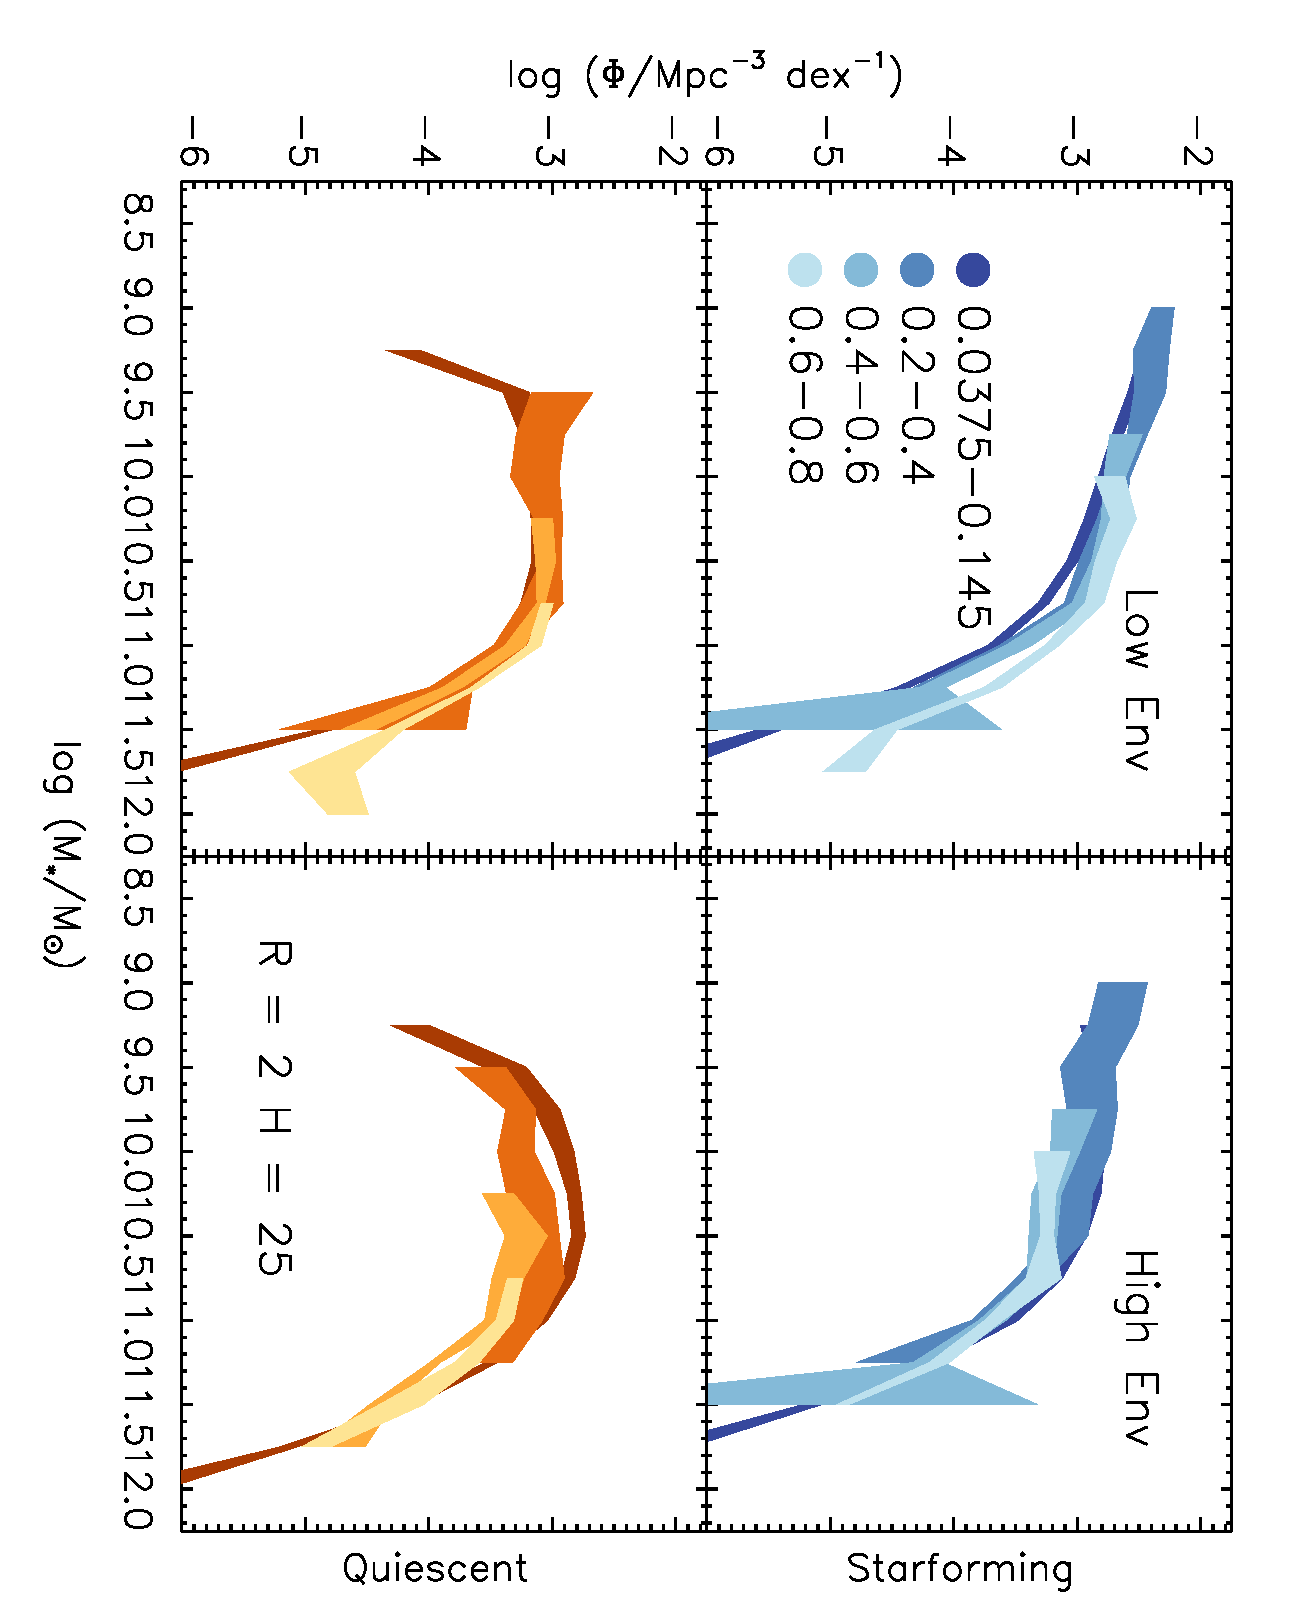
\epsfig{file=fig_smf_cylr2h25_thresh75_bin0_25.eps,height=0.75\textwidth,angle=90}
     \caption{Evolution of stellar mass functions of star-forming (top) and quiescent (bottom) target galaxies in 
low (left) and high (right) environments from redshift range $z=0-0.8$. The environment of each galaxy  
was calculated using a cylindrical aperture size of $R=2\rm{Mpc}$ and $H=25\rm{Mpc}$ and  
classification based on the cut-offs specified in Table \ref{tab:aperture}. The SMFs use mass bins of 
width $\Delta \rm{log}(\mathcal{M}/\mathcal{M}_{\odot})=0.25$. In each panel we use shades of blue 
(star-forming) and orange (quiescent) to represent the SMF at different redshift, higher redshifts being
progressively lighter.}
    \end{center}
\end{figure*}

The EDP for the PRIMUS sample is derived from the same parent sample as the target galaxies. 
We restrict the PRIMUS EDP galaxies within the redshift range $0.2-0.8$ and divide them into redshift bins of width $\Delta z = 0.2$. 
For each of these redshift bins, we impose separate absolute magnitude limits ($M_{r,\rm{lim}}$) such 
that the cumulative number density of the sample ordered by $M_{g}$ is equal to the cumulative 
number density of the highest redshift bin with an empirically determined limit. 
First, to determine the highest redshift bin ($0.8-1.0$) limit we look at the $M_{g}$ distribution with bin size
$\Delta M_{g} = 0.25$ and select $M_{g,\rm{lim}}$ to be the $M_{g}$ value near the peak of the 
distribution where number density of the bins with fainter objects (greater $M_{g}$ value) are smaller
than the number density of the bin at $M_{g, \rm{lim}}$. 
We find this $M_{g, \rm{lim}}( 0.8 < z < 1.0)$ to be, conservatively, $M_{g} = -20.75$. 
With this value we then calculate the rest of the $M_{g, \rm{lim}}$s by finding the
$M_{g}$ value where the cumulative number density ordered by absolute magnitude of the redshift bins 
equals that of the the highest redshift bin at $M_{g, \rm{lim}}( 0.8 < z < 1.0)$. 
Note that when calculating the number densities, the number of galaxies takes into account the 
statistical weights (described in Section \ref{sec:primus} and \ref{sec:sdss}).

For the EDP of the SDSS-{\em GALEX} sample (hereafter referred to as the SDSS EDP), we do not use the parent sample of the data due to 
the geometry of the combined angular selection function of the SDSS VAGC and {\em GALEX}. 
Instead, since we are not interested in the $FUV, NUV$ values for the EDP, we just use the
SDSS VAGC where the SDSS-{\em GALEX} catalog is derived from. 
Furthermore, we impose a redshift limit $0.0375-0.145$ on the SDSS EDP sample as opposed 
to the redshift range of $0.01-0.2$ in \cite{Moustakas:2013aa}.
This is due to the lack of faint galaxies at $z \sim 0.2$ and the lack of bright 
galaxies at $z \sim 0.01$. 
In other words, the lower bound for the redshif range was empirically determined by the bright limit of 
the $M_{g}$ versus redshift distribution and the upper bound by the faint limit of the 
$M_{g}$ versus redshift distribution. 
The same fixed cumulative number density method is used on this SDSS EDP. 
Ultimately we use $M_{g,\rm{lim}} = -20.57$, $-20.73$, $-20.80$ and $-20.95$ for the redshift bins 
$0.06-0.145$, $0.2-0.4$, $0.4-0.6$, $0.6-0.8$, respectively. 
These absolute magnitude limits are illustrated in Figure \ref{fig:targetEDP}, which plots the absolute magnitude versus the redshift for the EDP galaxies and the target galaxies. 

Using the above definition of environment and the EDP galaxies, we obtain the environment for each of the target population galaxies by counting the number of EDP galaxies, 
$n_{env}$, within the fixed cylinder aperture surrounding it. 
Since we use apertures of different dimensions, we are interested in the relative densitites rather than the actual $n_{env}$ values.
Hence, we use the percentage rank of the galaxy environment to quantify overdense environments and underdense environments.
More specifically, for each of the redshift bins ($0.2-0.4$, $0.4-0.6$, $0.6-0.8$, and $0.8-1.0$) the $n_{env}$ values for all target galaxies in that bin are listed and assigned a percentage rank based on their position in the list: $n_{env} = 0$ corresponding to $0\%$ and the maximum $n_{env}$ for a target galaxy in the $z$-bin corresponding to $100\%$. 
Using these percentage ranks, each target galaxy is classified as high-, mid-, or low-environment based on the cut-offs specified in Table \ref{tab:aperture}. 
Target sample galaxies are classified as high-environment if its percentage rank lies within the top $20\%$ and as low-environment if its percentage rank lies within the bottom $20\%$. 
In Table \ref{tab:aperture}, apertures with radius $1 h^{-1} \rm{Mpc}$ have a low-eneivonrment cut-off of higher than $20\%$.
This is because over $20\%$ of target sample galaxies have $n_{env}=0$ such a smaller aperture size.
Hence we defined the low-environment percentage rank cut-off to contain all galaxies with $n_{env}=0$. 
In order to have a fair comparison for the different $z$-bins when using this aperture, the low-environment cut-off was selected as the lowest cut-off that includes all galaxies with $n_{env}=0$ for all $z$-bin.
More specific details for the high- and low-environment cut-offs are provided in Table \ref{tab:aperture}.

Similar fixed aperture methods have also been used in \cite{Croton:2005aa} for galaxies in the 2dF Galaxy Redshift Survey (\cite{Colless:2003aa}) and in \cite{Muldrew:2012aa} 
for a mock galaxy catalogue generated from embedding galaxies onto the Millenium Dark Matter Simulation (\cite{Springel:2005aa}). 
%Perhaps include a sentence that sums up everything in Croton and Muldrew? 

\subsection{Edge Effects} \label{sec:edgeeffect}
\begin{figure*}
    \begin{center}
        \leavevmode
        \label{fig:smf}
        \epsfig{file=fig_qf_cylr2h25_thresh75_bin0_25.eps,height=0.75\textwidth,angle=90}
        \caption{Evolution of the quiescent fraction for target galaxies in low (left) and (high) environments
from redshift range $z=0-0.8$. The QFs were calculated using the SMFs specificed in Figure \ref{fig:smf}. We use
lighter shades of orange for the QFs at higher redshifts.}
    \end{center}
\end{figure*}

One of the challenges in obtaining the galaxy environment using a fixed aperture method is accounting for the edge effects of the survey.
For the target galaxies located near the edge of the survey, part of the fixed aperture encompassing it will lie outside the survey regions. 
In this case, the $n_{env}$ will only reflect the galaxies which lie in the fraction of the aperture contained within the survey geometry.

In order to account for these edge effects, we use a Monte Carlo method to impose edge cuts on the target galaxy population. 
We first divide the target sample galaxies into $n_{bin}$ redshift bins, specified in Table \ref{tab:aperture}. 
For each of the bins we compute the angular separation, $\theta_{\rm{ap}}$ that corresponds to the radius of the aperture at the central redshift of the bin.
Then the target galaxies in each bin are matched up to a sample of $N_{ransack}=1,000,000$ points with arbitrary $RA$ and $Dec$ values within the target sample fields, 
hereafter referred to as the ransack sample (named based on the procedure used to construct them). 
We count the number of ransack points, $n_{\rm{ransack}}$, within $\theta_{\rm{ap}}$ for the target galaxies in each of the redshift bins.
$n_{\rm{ransack}}$ values for the target galaxies are then compared to the expected value:
\begin{equation} \label{eq:ransack}
E[n_{\rm{ransack}}] = \frac{N_{\rm{ransack}}}{A_{\rm{fields}}}\times {\pi \theta_{\rm{ap}}^2} \times f_{\rm{thresh}} 
\end{equation} 
where $A_{\rm{fields}}$ is the total angular area of the target fields and $f_{\rm{thresh}}$ is the fractional threshold for the edge effect cut-off, specified in Table 
\ref{tab:aperture}.
If $n_{\rm{ransack}}$ for a target galaxy is greater than $E[n_{\rm{ransack}}]$ then the target galaxy remains in the sample; otherwise, it is discarded. 

\section{Results}
In this section, we describe our calculation to obtain the stellar mass functions (SMF) and quiescent fraction (QF) using the stellar mass complete target population.
In Section \ref{sec:smf_const} we construct the non-parametric estimate of SMFs for star-forming and quiescent galaxies in redshift bins: $0.06-0.145$, $0.2-0.4$, 
$0.4-0.6$, $0.6-0.8$, and $0.8-1.0$.
Form these SMFs, we calculate the QFs in section \ref{sec:qf_const}.

\subsection{Stellar Mass Function} \label{sec:smf_const}
Our primary interest in the SMFs is to investigate the evolution of the quiescent fraction in different density environments over our redshift range. 
Hence, we first divide the target galaxy sample into quiescent and star-forming target samples using the classification scheme from Section \ref{sec:sfq}.
Both the quiescent and star-forming target samples are then divided into "high-environment","mid-environment", and "low-environment" based on their environment classification described in 
Section \ref{sec:environment}.
We use the five redshift bins described in \ref{target} to get a total of $30$ subsamples that are classified based on star-forming/quiescent, environment, and redshift.
For each of these subsamples, we calculate the SMFs and their errors. 

To calculate the SMFs we employ a non-parametric $1/{V_{\rm{max}}}$ estimator commonly used for galaxy luminosity functions, as done in \cite{Moustakas:2013aa} and discussed 
in the review \cite{Johnston:2011aa}. 
The differential SMF is given by the following equation:
\begin{equation} \label{eq:phi}
\Phi(\rm{log}\: \mathcal{M}) \Delta(\rm{log} \:\mathcal{M}) = \sum\limits_{i=1}^{N} \frac{w_i}{V_{\rm{max,avail},i}}. 
\end{equation}
The equation above is the same as Equation 3. in \cite{Moustakas:2013aa} other than the use of $V_{\rm{max,avail}}$ instead than $V_{\rm{max}}$, which is used because of edge effect 
considerations along the edges of the survey. 
$w_i$ represnts the statistical weight of each galaxy $i$ and $\Phi(\rm{log}\: \mathcal{M}) \Delta(\rm{log}\: \mathcal{M})$ is the number of galaxies ($N$) per unit volume within the 
stellar mass range $[\rm{log} \:\mathcal{M}, \rm{log} \:\mathcal{M}+\Delta(\rm{log} \:\mathcal{M})]$.

$V_{\rm{max},i}$ is the maximum cosmological volume where it is possible to observe each galaxy $i$ given the apparent magnitude limits of the survey.
However in Section \ref{sec:edgeeffect} we remove the galaxies that lie on the edge of from the target sample. 
In doing so we reduce the maximum cosmological volume where a galaxy can be observed, thereby reducing $V_{\rm{max},i}$ to a what we will refer to as $V_{\rm{max,avail},i}$.

To calculate $V_{\rm{max,avail},i}$, we generate a sample of points with random $RA$, $Dec$, and $z$ (not to be confused with the ransack sample in Section \ref{sec:edgeeffect}) 
within the target fields and the redshift limits of the surveys.
We then impose the same edge effect cut-off used on the target galaxy population, described in Section \ref{sec:edgeeffect}, onto this random sample. 
For each redshift bin $j$ out of the $n_{\rm{bin}}$ redshift bins, we compute the fraction of the random points that remain in the bin after the points near the edges are removed: 
$f_{\rm{edge},j}$.
Finally we calculate: $V_{\rm{max,avail},i} = V_{\rm{max},i} \times f_{\rm{edge},j}$. 
The $V_{\rm{max},i}$ values in the equation above are computed following the method described in \cite{Moustakas:2013aa} with the same redshift-dependent $K$-correction 
from observed SED and luminosity evolution model.
For more details on computing $V_{\rm{max}}$ we refer readers to Section 4.2 in \cite{Moustakas:2013aa}. 

In order to calculate the uncertainty of the SMFs from the sample variance, we use a standard jackknife technique as done in \cite{Moustakas:2013aa}.
For the PRIMUS target galaxies, we calculate SMFs after excluding one of the target fields each time.
Note in these SMF calculations, the $1/V_{\rm{max},\rm{avail}}$ is corrected for the fact that excluding a field changes the total area of the survey.
Then using the calculated SMFs we calculate the uncertainty: 
\begin{equation}
\sigma^j = \sqrt{\frac{M-1}{M} \sum\limits_{k=1}^{M} (\Phi^j_k - \langle \Phi^j \rangle)^2}
\end{equation} 
$M$ in this equation is the number of jack knife SMFs in the mass bin; this value is different for each of the stellar mass bins since not all mass bins have galaxies from all five target fields.
$\langle \Phi^j \rangle$ is the mean number density of galaxies in each stellar mass bin for all of the jack knife $\Phi^j$s.

Since the SDSS-{\em GALEX} data are contained in one field, we first divide the field into a $30 \times 20$ rectangular grid and then only keep the sectors with at least $100$ galaxies in them. 
Then we use the same method as above to compute the uncertainties through the jack knife technique. 
The panels in the top two rows of Figure \ref{fig:smf} show the SMFs with uncertainties for all $30$ subsamples using aperture with dimensions $R_{\rm{ap}} = 1 \rm{Mpc}$ and $h_{\rm{ap}} = 50 \rm{Mpc}$.  

%Multiple apertures Additionally, we employ multiple apertures, as listed in Table \ref{tab:aperture}, since we are interested in probing the density environment at various scales. 
%Each aperture size will result in a different environment classification; so, $18$ SMFs are generated separately for every aperture we employ. 

\subsection{Quiescent Fraction} \label{sec:qf_const}
In the last section, we calculated the SMFs for all subsamples of the target galaxies classified by star-forming/quiescent, environment, and redshift. 
In this section, we use the $\Phi$ calculated for each subsample above to compute their respective $\rm{QF}$s: 
\begin{equation}
\rm{QF} = \frac{\Phi_{Q}}{\Phi_{SF}+\Phi_{Q}}.
\end{equation}
$\Phi_{Q}$ and $\Phi_{SF}$ are the total number of galaxies per unit volume in stellar mass bin $\Delta(\rm{log} \: \mathcal{M})$ (Equation \ref{eq:phi}) for the quiescent and star-forming subsamples, respectively.
A value for the $\rm{QF}$ is not assigned in stellar mass bins where either the star-formation subsample or the quiescent subsample do not have any galaxies. 
The bottom panels of Figure \ref{fig:smf} shows the $\rm{QF}$s for the different redshift bins and environment density classifications.

In order to compare the $\rm{QF}$s at different redshift for each of the environment classifications, we perform a linear least squares fit on the $\rm{QF}$ for all the $\rm{QF}$s. 
Then we use the value of the linear fit at an empirically selected fiducial mass $\rm{log} \: \mathcal{M}/\mathcal{M}_{\odot} = 10.5$ (using fiducial mass of $\rm{log} \: \mathcal{M}/
\mathcal{M}_\odot = 11.0$ does not noteably change the outcome).
These values are used to highlight and attempt to quantify the differences of the $\rm{QFs}$ at the different redshifts, Figure \ref{fig:qf}
%of the low redshift and low environemnt subsample.
%The slope obtained from this fit is then used to perform a lienar fit for the rest of the $\rm{QF}$s. 

The figures and analysis described in this paper are done using galaxy environment determined from a fixed aperture with $r_{\rm{ap}} = 1 \rm{Mpc}$ and $h_{\rm{ap}} = 50 \rm{Mpc}$.
The same analysis was repeated for various aperture dimensions: $r_{\rm{ap}} = 0.5, 1, 2, 3 \rm{Mpc}$ and $h_{\rm{ap}} = 25, 50 \rm{Mpc}$. 
Minor adjustments to the environment classification thresholds were adopted in these analyses for the smaller apertures ($r_{\rm{ap}} = 0.5, 1 \rm{Mpc}$ and $r_{\rm{ap}} = 25 \rm{Mpc}$).
The results obtained from using these different are consistent with the results displayed in this paper. 
\begin{figure}
    \begin{center}
        \leavevmode
        \epsscale{1.0}
        \plotone{fig_qffit_cylr2h25_thresh75_bin0_25.png}
        \label{fig:qf}
        \caption{Quiescent fraction at fiducial mass $\rm{log} (\mathcal{M}/\mathcal{M}_{\odot}) = 10.5$ for 
low (square) and high (circle) environments in the redshift range $z = 0 - 0.8$. The evolution of 
$f_{Q}(\mathcal{M}_{\rm{fid}})$ for galaxies in different environments shows an evolution over the redshift
range that is independent of environment density. Futhermore throughout the redshift range the difference in 
$f_{Q}(\mathcal{M}_{\rm{fid}})$ remains relatively constant and $ < 0.15$.}
    \end{center}
\end{figure}

\section{Discussion and Conclusions}
We have measured the SMFs and QFs using low redshift SDSS-{\em GALEX} galaxies and intermeidate redshift PRIMUS galaxies. 
Specifically we anlayzed the evolution of the QFs over the redshift range $0.0-1.0$ for galaxies in environment densities (Figure \ref{fig:qf}). 
We find that there is an expected increase in QF with decrease in the redshift for subsamples in all environment densities.
More importantly we find that the change in QF over redshift is independent of the environment and remains relatively equal for all environments. 

\begin{itemize}
    \item Comparison to other works. 
    \begin{itemize}
        \item Alberts et al. 2013 
    \end{itemize}
\end{itemize}

%
% References
%
\bibliography{PRIMUS}

\appendix
\begin{table*} %Will contain much more information on environments. 
  \caption{Fixed Cylindrical Aperture Dimensions}
  \label{tab:aperture}
  \begin{center}
    \leavevmode
    \begin{tabular}{llllll} \hline \hline              
  Radius (Mpc)          &Height (Mpc)      &$n_{bin}$   &Edgecut &High Env Threshold (galaxies) &Low Env Threshold (galaxies) \\ \hline 
  1.0 &50 &6 & 80\% & 1.5 & 0.0          \\
  2.0 &50 &6 & 75\% & 4.0 & 0.0          \\ \hline
  \multicolumn{6}{l}{}                                             \\       
    \end{tabular}
  \end{center}
\end{table*}

\subsection{Stellar Mass Function} \label{sec:smf_const}
\begin{figure*}
    \begin{center}
        \leavevmode
        \label{fig:smf}
        \epsscale{1.0}
        \plotone{fig_smf_cylr1h25_thresh80_bin0_25.png}
        \caption{SMF for $r_{\rm{ap}}=1 \rm{Mpc}$ and $h_{\rm{ap}}=25 \rm{Mpc}$}
    \end{center}
\end{figure*}

\begin{figure*}
    \begin{center}
        \leavevmode
        \label{fig:smf}
        \epsscale{1.0}
        \plotone{fig_qf_cylr1h25_thresh80_bin0_25.png}
        \caption{QF for $r_{\rm{ap}}=1 \rm{Mpc}$ and $h_{\rm{ap}}=25 \rm{Mpc}$}
    \end{center}
\end{figure*}

\begin{figure*}
    \begin{center}
        \leavevmode
        \epsscale{1.0}
        \plotone{fig_qffit_cylr1h25_thresh80_bin0_25.png}
        \label{fig:qf}
        \caption{QF at fiducial mass for $r_{\rm{ap}}=2 \rm{Mpc}$ and $h_{\rm{ap}}=50 \rm{Mpc}$}
    \end{center}
\end{figure*}

\end{document}
